\documentclass[letterpaper,addpoints,answers]{exam}
\usepackage{graphicx}
\usepackage{multicol}
\usepackage{wrapfig}
\usepackage{vwcol}
\usepackage{tikz}
\usetikzlibrary{scopes}

\makeatletter
\def\grd@save@target#1{%
  \def\grd@target{#1}}
\def\grd@save@start#1{%
  \def\grd@start{#1}}
\tikzset{
  grid with coordinates/.style={
    to path={%
      \pgfextra{%
        \edef\grd@@target{(\tikztotarget)}%
        \tikz@scan@one@point\grd@save@target\grd@@target\relax
        \edef\grd@@start{(\tikztostart)}%
        \tikz@scan@one@point\grd@save@start\grd@@start\relax
        \draw[minor help lines] (\tikztostart) grid (\tikztotarget);
        \draw[major help lines] (\tikztostart) grid (\tikztotarget);
        \grd@start
        \pgfmathsetmacro{\grd@xa}{\the\pgf@x/1cm}
        \pgfmathsetmacro{\grd@ya}{\the\pgf@y/1cm}
        \grd@target
        \pgfmathsetmacro{\grd@xb}{\the\pgf@x/1cm}
        \pgfmathsetmacro{\grd@yb}{\the\pgf@y/1cm}
        \pgfmathsetmacro{\grd@xc}{\grd@xa + \pgfkeysvalueof{/tikz/grid with coordinates/major step x}}
        \pgfmathsetmacro{\grd@yc}{\grd@ya + \pgfkeysvalueof{/tikz/grid with coordinates/major step y}}
        \foreach \x in {\grd@xa,\grd@xc,...,\grd@xb}
        \node[anchor=north] at (\x,\grd@ya) {\pgfmathprintnumber{\x}};
        \foreach \y in {\grd@ya,\grd@yc,...,\grd@yb}
        \node[anchor=east] at (\grd@xa,\y) {\pgfmathprintnumber{\y}};
      }
    }
  },
  minor help lines/.style={
    help lines,
    gray,
    line cap =round,
    xstep=\pgfkeysvalueof{/tikz/grid with coordinates/minor step x},
    ystep=\pgfkeysvalueof{/tikz/grid with coordinates/minor step y}
  },
  major help lines/.style={
    help lines,
    line cap =round,
    line width=\pgfkeysvalueof{/tikz/grid with coordinates/major line width},
    xstep=\pgfkeysvalueof{/tikz/grid with coordinates/major step x},
    ystep=\pgfkeysvalueof{/tikz/grid with coordinates/major step y}
  },
  grid with coordinates/.cd,
  minor step x/.initial=.5,
  minor step y/.initial=.2,
  major step x/.initial=1,
  major step y/.initial=1,
  major line width/.initial=1pt,
}
\makeatother



\begin{document}

\begin{coverpages}
 \large\bfseries
 
 \noindent 
 Physics 107: Physics for Life-Sciences

 \vspace{2ex}
 \noindent
 Final Exam: December 8, 2014

 \vspace{3ex}
 \noindent 
 This test is administered under the rules and regulations of the honor code of the College of William \& Mary.

 \vspace{2ex}
 \noindent 
 Name:\enspace\makebox[2.3in]{\hrulefill} \\

 \noindent 
 Signature:\enspace\makebox[2in]{\hrulefill} \\

 \vspace{5ex}
 \noindent 
 Instructions:
 \begin{itemize}
  \item This is a closed book, closed notes test.
  \item Calculators are permitted, but not laptops or cell phones. Devices with wireless connections are not allowed.
  \item Start your work from the fundamental equations on the formula sheet, and derive any additional expressions that you may need.
  \item Circle your answer for each part of each problem. 
  \item Clearly mark out any work that you wish the grader to disregard.  Do not waste your time erasing.
  \item Your work will be graded based on your ability to write down a logical and organized solution grounded in the correct assessment of the physics of a situation. No credit will be given for an answer that is not justified by a logical solution or where that justification is not organized or readable.
  \item Partial credit will be given up to the point where your solution departs from a correct analysis of the physics involved for any given part of a problem.
 \end{itemize}

 \pagebreak

 \begin{center}
  \gradetable[v][questions]
 \end{center}
 
\end{coverpages}


\begin{questions}

\question[5]
You are operating a small remote controlled toy car on the sidewalk along Jamestown Road. As you are standing on the sidewalk, the speed of the toy car relative to you is plotted below.  What is the displacement of the toy car between 0\,s and 13\,s?

\begin{center}
 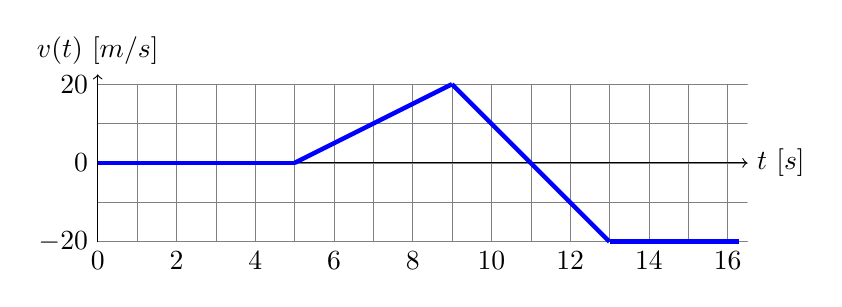
\begin{tikzpicture}[xscale=0.5,yscale=0.05,grid with coordinates/major step x=2,grid with coordinates/minor step x=1,grid with coordinates/major step y=20,grid with coordinates/minor step y=10,grid with coordinates/major line width=0.2pt]
  \draw (0,-20) to[grid with coordinates] (16.5,20);
  \draw[->] (0,0) -- (16.5,0) node[right] {$t~[s]$};
  \draw[->] (0,-20) -- (0,22.5) node[above] {$v(t)~[m/s]$};
  \draw[ultra thick,color=blue] (0.0,0.0) -- (5.0,0.0);
  \draw[ultra thick,color=blue] (5.0,0.0) -- (9.0,+20.0);
  \draw[ultra thick,color=blue] (9.0,+20.0) -- (13.0,-20.0);
  \draw[ultra thick,color=blue] (13.0,-20.0) -- (16.3,-20.0);
 \end{tikzpicture}
\end{center}
\begin{checkboxes}
 \choice -20\,m
 \choice 4\,m
 \choice 40\,m
 \choice 80\,m
 \choice 300\,m
\end{checkboxes}

\question[5]
A ball is thrown straight up, reaches a maximum height, and then falls back downward. Which of the following are true when it reaches its maximum height?
\begin{checkboxes}
 \choice Its velocity and its acceleration are zero.
 \choice Its velocity is zero and its acceleration points upward.
 \choice Its velocity is zero and its acceleration points downward.
 \choice Its velocity points downward and its acceleration points upward.
 \choice Its velocity and its acceleration point downward.
\end{checkboxes}

\question[5]
A 2.2\,kg pumpkin is going to be dropped from the top of the Wren building to the sidewalk below. The height is 15.5\,m above the sidewalk. You want to set a delay timer on your camera for taking a picture upon impact. You want to determine how long it takes for the pumpkin to hit the ground after it was dropped. Select the relationship that will most directly lead you to the result using the given information?
\begin{checkboxes}
 \choice $v = v_0 + a \Delta t$
 \choice $\Delta KE + \Delta PE = W_{nc}$
 \choice $\Delta y = v_0 \Delta t + \frac{1}{2} a \Delta t^2$
 \choice $W = F d \cos \theta$
 \choice $v^2 = v_0^2 + 2 a \Delta y$
 \choice $\Delta PE_g = m g \Delta y$
\end{checkboxes}

\pagebreak

\question[5]
A merry-go-round on a playground can be thought of as a rotating disk of 52\,kg with a diameter of 2.52\,m. A girl on the playground starts from rest and has the merry-go-round spinning at 0.2 revolutions per second when she lets go after a quarter turn. She is standing next to it and no one is on the merry-go-round while it spins. What is the velocity of a point at the outer edge of the merry-go-round after it gets to its final speed?
\begin{center}
 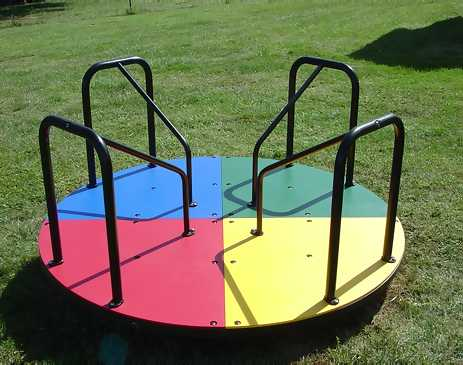
\includegraphics[width=0.35\textwidth]{merry_go_round}
\end{center}
\begin{checkboxes}
 \choice 3.17\,m/s
 \choice 1.58\,m/s
 \choice 0.79\,m/s
 \choice 0.50\,m/s
 \choice 0.25\,m/s
\end{checkboxes}

\question[5]
Explain \textbf{in words only} the difference between a stable and an unstable equilibrium. Limit yourself to at most three sentences.

\pagebreak

\question
Road Runner's revenge.  Wile E.~Coyote is on the vertical front of a train that is accelerating. He is not standing on anything and is not holding on to anything. He is being held up solely by the frictional force between him and the front of the accelerating train. Coyote has a mass of 20.0\,kg, and the coefficient of static friction is 0.45 for this situation.

\begin{center}
 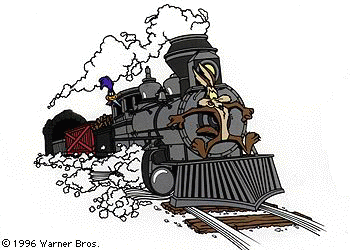
\includegraphics[width=0.5\textwidth]{train}
\end{center}

\begin{parts}
 \part[5] Draw the free body diagram for the coyote.
 \vspace{\stretch{1}}
 \part[5] Write down the components of the important vectors on the coyote in terms of their \emph{magnitudes and angles}. If the magnitudes and angles of these vectors are unknown, then define variables to break down the components in the format $(F \cos\theta, F\sin\theta)$.
 \vspace{\stretch{1}}
 \part[10] Using Newton's laws determine the minimum acceleration required for the coyote to not slip down the front of the train?
 \vspace{\stretch{1}}
\end{parts}

\pagebreak

\question
You have been hired by the Police Department to examine their new pistols. They have asked you to determine the velocity of the bullets when they leave the handgun. To test this you fire a standard 5.17\,g bullet toward a wood block hanging from a rope (called a ballistic pendulum). When the bullet hits the block is embeds itself in the wood. You observe that the block swings upward after the collision. When you do your experiment you note that the 2.27\,kg block swings to a height of 0.268\,m above its original hanging position.

\begin{center}
 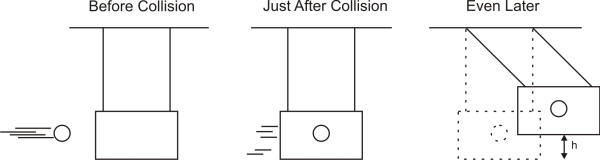
\includegraphics[width=0.6\textwidth]{ballistic_pendulum}
\end{center}

\begin{parts}
 \part[5] What is the potential energy of the block and bullet when it is at its highest position?
 \vspace{\stretch{1}}
 \part[5] What is the speed of the block and the bullet just after the bullet hits the block?
 \vspace{\stretch{1}}
 \part[5] What is the speed of the bullet before the collision?
 \vspace{\stretch{1}}
\end{parts}

\pagebreak

\question
Even when the head is held erect, as in the figure below, its center of mass is not directly over the principal point of support (the atlanto-occipital joint). The muscles in the back of the neck must therefore exert a force to keep it erect. That is why your head falls forward when you fall asleep in class. The perpendicular distance between the line of action for the weight of the head and the pivot point is $r_{W\perp} = 2.1$\,cm and the perpendicular distance between the line of action for the force the muscles exert on the head and the pivot point is $r_{M\perp} = 5.6$\,cm. Assume the weight of the head is 50 N.
\begin{center}
 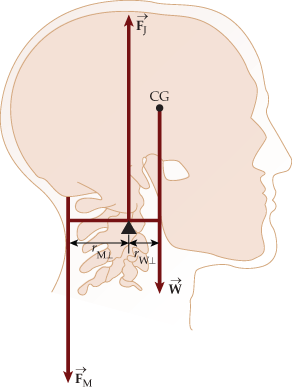
\includegraphics[width=0.3\textwidth]{head}
\end{center}
\begin{parts}
 \part[10] What is the force exerted by the muscles?
 \vspace{\stretch{1}}
 \part[10] What is the force on the point of support?
 \vspace{\stretch{1}}
\end{parts}


\pagebreak

\question
You place a beaker that is two-thirds full of water with a density of $\rho_{H_2O} = 1000$\,kg/m$^3$ on a laboratory scale. You then use a light-weight cord to suspend an aluminum object with density $\rho_{Al} = 2700$\,kg/m$^3$ in the water. The object is completely submerged, and none of the water spills out of the beaker. The reading on the scale changes by 0.054\,kg.
\begin{parts}
 \part[10] What is the volume of the object?
 \vspace{\stretch{1}}
 \part[10] What is the tension in the cord while the object is submerged?
 \vspace{\stretch{1}}
\end{parts}

\question
A long horizontal hose of diameter 0.016\,m is connected to a faucet. At the other end, there is a nozzle of diameter 0.004\,m. Water squirts from the nozzle at a velocity of 38\,m/s. Assume that the water has no viscosity or other form of energy dissipation, and that the density of water is 1000\,kg/m$^3$.
\begin{parts}
 \part[5] What is the velocity of the water within the hose?
 \vspace{\stretch{1}}
 \part[5] What is the pressure differential between the water in the hose and water in the nozzle?
 \vspace{\stretch{1}}
\end{parts}

\pagebreak

\question
A spring has a length of 0.333\,m when a 0.300\,kg mass hangs from it, and a length of 0.750\,m when a 3.00\,kg mass hangs from it.  With the mass of 3.00\,kg attached it is set in simple harmonic motion by pulling it down an additional 0.125\,m and letting it go from there.
\begin{parts}
 \part[5] What is the force constant of the spring?
 \vspace{\stretch{1}}
 \part[5] What will be the period of oscillations?
 \vspace{\stretch{1}}
\end{parts}

\question
A large housefly 3.0 meters away from you makes a noise of 40\,dB.
\begin{parts}
 \part[5] How many decibels would the housefly make if it were 30 centimeters away?
 \vspace{\stretch{1}}
 \part[5] With a noise level of 40\,dB, how much energy falls on your eardrum, which has a diameter of 1.0\,cm, in one minute?
 \vspace{\stretch{1}}
\end{parts}

\pagebreak

\question
The William \& Mary Pep Band is moving towards you at 2\,m/s. A clarinet player is playing a perfect 185.0\,Hz note. Assume the speed of sound is 331\,m/s.
\begin{parts}
 \part[5] What frequency do you hear?
 \vspace{\stretch{1}}
 \part[5] What is the wavelength of the sound?
 \vspace{\stretch{1}}
 \part[5] Another clarinet player is standing still (\textit{i.e.} not marching) by the first player, and also plays a perfect 185.0\,Hz note.  What is the beat frequency that you hear?
 \vspace{\stretch{1}}
 \part[5] A clarinet is a tube that is open at both ends. If 185.0\,Hz is the fundamental frequency, what it the length of the clarinet?
 \vspace{\stretch{1}}
\end{parts}

\end{questions}

\pagebreak
 
 {\Large Possibly useful relations (please detach this page):}
  
 \fontseries{\seriesdefault}
 \begin{multicols}{2}
 \normalsize
 \noindent
 $\vec{v}_{avg} = \Delta\vec{x} / \Delta t$ \\
 $\vec{a}_{avg} = \Delta\vec{v} / \Delta t$ \\
 $v = v_0 + a t$ \\
 $v_{avg} = \frac{v_0 + v}{2}$ \\
 $x = x_0 + v_0 t + \frac{1}{2} a t^2$ \\
 $v^2 = v_0^2 + 2 a (x - x_0)$ \\
 $R = \frac{v_0^2}{g}\sin 2\theta$ \\
 $h = \frac{v_0^2}{2 g} \sin^2 \theta$ \\
 $\vec{F}_{net} = m \vec{a}$ \\
 $\vec{F}_{BA} = - \vec{F}_{AB}$ \\
 $\vec{W} = m \vec{g}$ \\
 $\vec{g} = 9.80\,$m/s$^2$ downward \\
 $0 \le f_s \le \mu_s N$ \\
 $f_k = \mu_k N$ \\
 $\frac{F}{A} = Y \frac{\Delta L}{L}$ \\
 $F_k = -k x$ \\
 $W = F d \cos\theta$ \\
 $W_{net} = -\Delta PE = \Delta KE$ \\
 $KE = \frac{1}{2} m v^2$ \\
 $PE_k = \frac{1}{2} k x^2$ \\
 $PE_g = m g h$ \\
 $KE_i + PE_i + W_{nc} = KE_f + PE_f$ \\
 $P = \frac{W}{\Delta t}$ \\
 $\hbox{Eff} = \frac{W_{out}}{E_{in}}$ \\
 $F_G = G \frac{m M}{r^2}$ \\
 $G = 6.67 \times 10^{-11}\,$N $\cdot$ m$^2$ / kg$^2$ \\
 $\vec{I} = \vec{F}_{avg} \Delta t$ \\
 $\vec{p} = m \vec{v}$ \\
 $\vec{F}_{net} = \frac{\Delta \vec{p}}{\Delta t}$ \\
 $v_1 - v_2 = v'_2 - v'_1$ \\
 $\theta = \frac{s}{r}$ \\
 $v = r \omega$ \\
 $f = \frac{1}{T}$ and $\omega = 2 \pi f = \frac{2 \pi}{T}$ \\
 $a_c = \frac{v^2}{r} = r \omega^2$ \\
 $F_c = m\frac{v^2}{r} = m r \omega^2$ \\
 $KE_{trans} = \frac{1}{2} m v^2$ \\
 $KE_{rot} = \frac{1}{2} I \omega^2$ \\
 $I_{point} = M R^2$ \\
 $I_{disk} = \frac{1}{2} M R^2$ \\
 $I_{sphere} = \frac{2}{5} M R^2$ \\
 $\tau = r F \sin\theta = r_\perp F$ \\
 $\omega = \Delta \theta/\Delta t$ \\
 $\alpha = \Delta \omega/\Delta t$ \\
 $\tau = I \alpha$ \\
 $L = I \omega$ \\
 $\tau = \frac{\Delta L}{\Delta t}$ \\
 $P = \frac{F}{A}$ \\
 $P_{gauge} = P - P_{atm}$ \\
 $\rho = \frac{M}{V}$ \\
 $Q = \frac{\Delta V}{\Delta t} = A v$ \\
 $Q = \frac{\Delta P \pi r^4}{8 \eta L}$ \\
 $\hbox{Power} = P Q$ \\
 $A \cdot v = \hbox{constant}$ \\
 $P + \rho g y + \frac{1}{2} \rho v^2 = \hbox{constant}$ \\
 $F_B = \rho g V_{displaced}$ \\
 $F_{ST} = \gamma L$ \\
 $P = \frac{4 \gamma}{r}$ \\
 $h = \frac{2 \gamma}{\rho g r}$ \\
 $N_R = \frac{\rho v L}{\eta} = \frac{2 \rho v r}{\eta}$ \\
 $x_{rms} = \sqrt{2 D t}$ \\
 $x(t) = A \cos \omega t$ and $x_{max} = A$ \\
 $v(t) = - A \omega \sin \omega t$ and $v_{max} = A \omega$ \\
 $a(t) = - A \omega^2 \cos \omega t$ and $a_{max} = A \omega^2$ \\
 $E = \frac{1}{2} k x^2 + \frac{1}{2} m v^2 = \frac{1}{2} k x_{max}^2 = \frac{1}{2} m v_{max}^2$ \\
 $v = \sqrt{T/\mu}$ with $\mu = \frac{m}{L}$ \\
 spring: $\omega = \sqrt{k/m}$ \\
 pendulum: $\omega = \sqrt{g/\ell}$ \\
 $y(x,t) = A \cos (\omega t \pm k x)$ with $-$ for left-moving wave \\
 $\omega = \frac{2 \pi}{T}$ and $k = \frac{2 \pi}{\lambda}$ \\
 $v = \lambda f = \frac{\omega}{k}$ \\
 $v_{sound} = 331\,\hbox{m/s} \sqrt{\frac{T}{273\,K}}$ \\
 string: $\lambda_n = \frac{2 L}{n}$, $f_n = \frac{n v}{2 L}$ with $n = 1,2,3,\ldots$ \\
 open-open: $\lambda_n = \frac{2 L}{n}$, $f_n = \frac{n v}{2 L}$ with $n = 1,2,3,\ldots$ \\
 open-closed: $\lambda_n = \frac{4 L}{n}$, $f_n = \frac{n v}{4 L}$ with $n = 1,3,5,\ldots$ \\
 $f_{obs} = f_{src} \frac{v}{v \pm v_{src}}$ with $-$ for src moving towards obs \\
 $f_{obs} = f_{src} \frac{v \pm v_{obs}}{v}$ with $+$ for obs moving towards src \\
 $f_{beat} = |f_1 - f_2|$ \\
 $I = \frac{P}{A} = \frac{P}{4 \pi r^2}$ \\
 $\beta = 10 \log \frac{I}{I_0}$ in dB with $I_0 = 10^{-12}$\,W/m$^2$\\
 $1\,\hbox{atm} = 10^5\,\hbox{Pa} = 760\,\hbox{mm}\cdot\hbox{Hg}$ \\
 $\rho_{water} = 10^3\,\hbox{kg}/\hbox{m}^3$ \\
 $1\,\hbox{cal} = 4.186$\,J and $1\,\hbox{Cal} = 1000$\,cal \\ 
 $\cos\theta = \hbox{adjacent}/\hbox{hypotenuse}$ \\
 $\sin\theta = \hbox{opposite}/\hbox{hypotenuse}$ \\
 $\tan\theta = \sin\theta / \cos\theta$ \\
 $x = \frac{-b \pm \sqrt{b^2 - 4 a c}}{2 a}$ \\

 \end{multicols}

\end{document}
